\documentclass[11pt]{article}
\usepackage{graphicx,color}
\usepackage{nth}

\setlength{\textwidth}{6.5in}
\setlength{\textheight}{8.0in}
\setlength{\oddsidemargin}{0in}
\setlength{\evensidemargin}{0in}
\setlength{\parskip}{2ex}
\setlength{\parindent}{0in}

%To display answers, replace "white" with "red" here;
\newcommand{\answer}[1]{\color{white}#1}

\begin{document}

\begin{enumerate}

\item The incubation time for Rhode Island Red chicks is normally distributed with a mean of $\mu = 21$ days and a standard deviation of about $\sigma =1$ day.  If 1000 eggs are being incubated, how many chicks do we expect to hatch

	\begin{enumerate}
	\item on day 21 or after?
	
	{\answer Since $\mu = 21$, the percentage of the eggs that will hatch at that time or greater is 50\%.  So, that is 500 of the eggs.}
	
	\item between 20 and 21 days? 
	
	{\answer Since $\mu = 21$ and $\sigma =1$, we are looking at the percentage of the eggs in the interval $\mu-\sigma$ to $\mu$ which is 34\%.  So, that is 340 of the eggs.}
	
	\item between 22 and 23 days?
	
	{\answer Since $\mu = 21$ and $\sigma=1$, we are looking at the percentage of eggs in the interval $\mu+\sigma$ and $\mu + 2\sigma$ which is 13.5\%.  So, that is 135 of the eggs.}
	
	\item between 19 and 22 days?
	
	{\answer Since $\mu = 21$ and $\sigma=1$, we are looking at the percentage of eggs in the interval $\mu-2\sigma$ and $\mu + \sigma$ which is 81.5\%.  So, that is 815 of the eggs.}
	
	\end{enumerate}

\item The Empirical Rule tells us the percentage of data values that lie within certain intervals about the mean when we have a normal distribution as follows.

\begin{center}
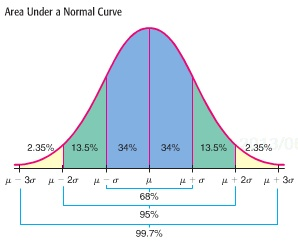
\includegraphics[scale=0.5]{WS10_NormalArea.jpg}
\end{center}

	\begin{enumerate}
	\item According to Chebyshev's Theorem, what is the minimum percentage of data that must lie within the interval $\mu-2\sigma$ to $\mu + 2\sigma$?  How does this compare to the results for the Empirical Rule?
	
	{\answer The result of Chebysev's Theorem is that at least $1-\frac{1}{2^2} = 75\%$ of the data fall within in the interval...and this is true for {\em any} data distribution.  \\
	For a normal distribution, the Empirical Rule shows us that there is approximate 95\% of the data falling within that same range.}
	
	\item The diagram for the Empirical Rule only accounts for 99.7\% of the data values.  Where do the remaining 0.3\% of the data fall?
	
	{\answer The remaining 0.3\% must lie outside the interval from $\mu-3\sigma$ to $\mu + 3\sigma$...That is, those data values lie fall out in the tails of the distribution.  Additionally, since the distribution is symmetric, half of them (or 0.15\%) lie below $\mu-3\sigma$ and the other half lie above $\mu + 3\sigma$.} 
	
	\item Keeping in mind that remaining 0.3\% of the data, what percentage of the data values lie to the left of $\mu-\sigma$?
	
	{\answer Add 13.5\%, 2.35\%, and 0.15\% to get 16\%. 
	
	Note that equivalently, since we know that 50\% lie to the left of the mean $\mu$ and 34\% lie between $\mu-\sigma$ and $\mu$, that leaves 16\% lying to the left of $\mu-\sigma$. }
	
	\item Keeping in mind that remaining 0.3\% of the data, what percentage of the data values lie to the left of $\mu+2\sigma$? 
	
	{\answer Add 13.5\%, 34\%, 34\%, 13.5\%, 2.35\%, and 0.15\% to get 97.5\%.
	
	Note that equivalently, since we know that 50\% lie to the left of the mean $\mu$ and $34\%+13.5\%$ lie between $\mu$ and $\mu+2\sigma$, that total is 97.5\% lying to the left of $\mu+2\sigma$. } 

	\end{enumerate}

\item In preparation for Sections 6.2 and 6.3 (of Brase and Brase), suppose the mean of a normal distribution is $\mu = 75$ with a standard deviation of $\sigma = 8$.  For each of the following values of the random variable $x$, determine whether $x$ is above or below the mean and then determine the number of standard deviations away from the mean that $x$ lies.  (Note that your second answer could be a fraction or decimal number.)

	\begin{enumerate}
	\item $x=83$ 
	
	{\answer $x=83$ is above the mean of $\mu = 75$.  Specifically, $\frac{83-75}{8} = 1$.  So, $x$ is 1 standard deviation above the mean.}
	\item $x=51$ 
	
	{\answer $x=51$ is below the mean of $\mu = 75$.  Specifically, $\frac{51-75}{8} = -3$ .  So, $x$ is 3 standard deviations below the mean.}
	\item $x=79$ 
	
	{\answer $x=79$ is above the mean of $\mu = 75$.  Specifically, $\frac{79-75}{8} = 0.5$.  So, $x$ is $0.5$ standard deviations above the mean.}
	\item $x=65$ 
	
	{\answer $x=65$ is below the mean of $\mu = 75$.  Specifically, $\frac{65-75}{8} = -1.25$.  So, $x$ is $1.25$ standard deviations below the mean.}
	\end{enumerate}

\item Hydraulic pressure in the main cylinder of the landing gear of a commercial jet is very important for a safe landing.  In-flight landing tests show that the actual pressure in the main cylinders is variable (approximately normal) with a mean of 819 pounds per square inch and a standard deviation of 23 pounds per square inch, which are considered safe.

Two different planes were tested with 10 test-landings.  


\begin{tabular}{l|cccccccccc}
\hline 
landing number for plane A& 1& 2 & 3 & 4 & 5 & 6 & 7 & 8 & 9 & 10 \\
\hline
pressure & 870 & 855 & 830 & 815 & 847 & 836 & 825 & 810 & 792 & 820 \\
\hline
\end{tabular}

\begin{tabular}{l|cccccccccc}
\hline 
landing number for plane B& 1& 2 & 3 & 4 & 5 & 6 & 7 & 8 & 9 & 10 \\
\hline
pressure & 865 & 850 & 841 & 820 & 815 & 789 & 801 & 765 & 730 & 725 \\
\hline
\end{tabular}

	\begin{enumerate}
	\item  Is the pressure for Plane A ``in control" or not?  If not, describe the specific out-of-control signals present. 
	
	{\answer Out of control Signal 1: $\mu -3\sigma = 750$ and $\mu +3\sigma = 888$.  No values fall outside that range. Out of control Signal 2 : $\mu = 819$.  There are no more than 3 consecutive values above $\mu$ and no more than 2 consecutive values below $\mu$. Out of control Signal 3: $\mu -2\sigma = 773$ and $\mu +2\sigma = 865$.  There is only 1 value that lies beyond either end of that range, so certainly not 2 of 3 consecutive values do. There are no out-of-control warning signals present for Plane A.} 
	
	\item  Is the pressure for Plane B ``in control" or not?  If not, describe the specific out-of-control signals present.
	
	{\answer Out of control Signal 1: $\mu -3\sigma = 750$ and $\mu +3\sigma = 888$.  There are two values that fall below 750. Out of control Signal 2 : $\mu = 819$.  There are no more than 4 consecutive values above $\mu$ and no more than 6 consecutive values below $\mu$. Out of control Signal 3: $\mu -2\sigma = 773$ and $\mu +2\sigma = 865$.  The last three values recorded lie below 773, so there are two occasions of 2 out of 3 consecutive values flying beyond the $2\sigma$ level on the same side. There are two out-of-control warning signals present for Plane B.} 

	\end{enumerate}
	

\item Let $x$ be a random variable with a normal distribution with mean $\mu = 15$ and standard deviation $\sigma = 4$.  Find the indicated probability.

	\begin{enumerate}
	\item $P(x \leq 12)$ 
	
	{\answer $\texttt{normalcdf(-1E99,12,15,4)} =  0.2266272794 \approx 22.66\%$
	} 
	
	\item $P(x > 10)$ 
	
	{\answer $\texttt{normalcdf(10,1E99,15,4)} =  0.894350161 \approx 89.44\%$
	} 
	
	\item $P(15 \leq x \leq 20)$ 
	
	{\answer $\texttt{normalcdf(15,20,15,4)} =  0.3943501605 \approx 39.44\%$
	} 
	
	\item $P(8 < x < 22)$ 
	
	{\answer $\texttt{normalcdf(8,22,15,4)} =  0.9198817729 \approx 91.99\%$
	} 
	\end{enumerate}

\item Find the $z$-value described.

	\begin{enumerate}
	
	\item Find $z$ such that 5.2\% of the standard normal curve lies to the left of $z$.  
	
	{\answer This is a left-tail area, so $z = \texttt{invNorm(0.052, 0, 1) = -1.625763385}$.
	} 

	\item Find $z$ such that 5\% of the standard normal curve lies to the right of $z$.  
	
	{\answer Since this is a right-tail area, we can first translate this to a left-tail area by equating ``5\% to the right of $z$" with ``95\% to the left of $z$."  
	
	Then $z = \texttt{invNorm(0.95,0,1)} = 1.644853626$. 
	
	Note that alternatively, symmetry can be used with  $\texttt{invNorm(0.05,0,1) = -1.644853626}$ to conclude $z=1.644853626$.
	} 

	\item Find $z$ such that 95\% of the standard normal curve lies between $-z$ and $+z$. 
	
	{\answer To use \texttt{invNorm}, we must first translate this to a left-tail area problem.  If 95\% of the area lies {\em between} $-z$ and $+z$, then we can equate this to 97.5\% lies to the left of $+z$.  
	Then $z = \texttt{invNorm(0.975, 0, 1)} = 1.959963986$, and $-z = -1.959963986$.
	} 
	
	%--
	\end{enumerate}
	
\item Suppose that the scores for a Chemistry midterm had a normal distribution with mean $\mu = 71.4$ and a standard deviation of $\sigma = 8.3$.

	\begin{enumerate}
	
	\item Find the exam score for a student that scored in the \nth{80} percentile. 
	
	{\answer The \nth{80} percentile refers to the score where 80\% of the class earned that score or below.  That is, the left-tail area related to this score is 80\%. So, $x = \texttt{invNorm(0.80, 71.4, 8.3)} = 78.38545624 \approx 78.4$.
	} 
	
	\item Find the exam score for a student that scored in the $25^{th}$ percentile. 
	
	{\answer The $25^{th}$ percentile refers to the score where 25\% of the class earned that score or below.  That is, the left-tail area related to this score is 25\%. So, $x = \texttt{invNorm(0.25, 71.4, 8.3)} = 65.80173508 \approx 65.80$.
	} 
	
	\item Find the exam score for a student who score lower than 60\% of the class. 
	
	{\answer Scoring lower than 60\% of the class implies that the right-tail area related to this score is 60\%.  However, since the \texttt{invNorm} function requires the left-tail area as its input, we must first translate this problem to the left-tail area of 40\%.	Then,  $x = \texttt{invNorm(0.40, 71.4, 8.3)} = 69.29721906 \approx 69.30$.
	} 
	\end{enumerate}

	

\item Suppose the distribution of heights of American men (20 years of age and older) is approximately normal with a mean of 69.4 inches and a standard deviation of 3 inches.

	\begin{enumerate}
	
	\item What is the $z$ value for a height of 6 feet? 
	
	{\answer First we convert 6 feet to 72 inches. Then $z = \frac{72-69.4}{3} = 0.86666667.$}
	
	\item What percentage of American men (20 years of age and older) are shorter than 6 feet?
	
	{\answer   We can use \texttt{normalcdf}.  
	$$P(z < 0.86666667) = \texttt{normalcdf(-1E99, 0.86666667, 0, 1)} = 0.8069377087 \approx 80.69\%$$}
	
	\item What is the $z$ value for a height of 6 feet 4 inches?
	
	{\answer First we convert 6 feet 4 inches to 76 inches.	Then $z = \frac{76-69.4}{3} = 2.2$.} 
	
	\item What percentage of American men (20 years of age and older) are taller than 6 feet 4 inches?
	
	{\answer  We can use \texttt{normalcdf}. $$P(z > 2.2) = \texttt{normalcdf(2.2, 1E99, 0, 1)} = 0.0139033989 \approx 1.39\%$$}
	
%	\item If we were to choose a random sample of 10 American men (20 years of age and older), what is the probability that at two or more of them are taller than 6 feet? \\
%	{\answer  Because the population of American men is so large, we can use the binomial experiment model to answer this question with $n = 10$, $r= 2$, and $p = 1 - 0.8069374216 =0.1930625784$ (as we just found in part (a)).  $$P(r \geq 2) = 1 - P(r\leq 1) = 1 - \texttt{binomcdf(10, 0.1930625784, 1)} =0.6028789926 \approx 60.29\%$$}
%	\item How many American men (20 years of age and older) do you need in your sample to be 99\% certain that you have at two or more who are taller than 6 feet? \\
%	{\answer This is a quota problem, where we are looking for $P(r \geq 2) \geq 0.99$.  So, we want $$1 - \texttt{binomcdf(n, 0.1930625784, 1)} = 0.99.$$  Using the \texttt{TABLE} of the TI-84, we can see that $n=32$ is the minimum sample size we need to reach that 99\% probability.}
	\vspace{0.5cm}
	\end{enumerate}

%Section 6.3 #30
\item Accrotime is a manufacturer of quartz crystal watches. Accrotime researchers have shown that the watches have an average life of 28 months before certain electronic components deteriorate, causing the watch to become unreliable.  The standard deviation of watch lifetimes is 5 months, and the distribution of lifetimes is normal.

	\begin{enumerate}
	
	\item If Accrotime guarantees a full refund on any defective watch for 2 years, what percentage of total production will the company expect to replace? 
	
	{\answer First we need to make sure all time intervals are measured in the same units.  So, we are looking for the percentage of watches that are expected to fail in 24 months or fewer. 
	
	$P(x\leq 24) = \texttt{normalcdf(-1E99, 24, 28, 5)} = 0.2118553337$.  This means that the company should expect to replace about 21.19\% of its watches.
	} 

	\item If Accrotime does not want to make refunds on more than 12\% of the watches it makes, how long should the guarantee period be (to the nearest month)? 
	
	{\answer Certainly, it is shorter than 24 months, since that led to 21.19\% replaced.  To determine a more precise number of months, we can use \texttt{invNorm} where we are looking for a left-tailed area equal to $0.12$. 
	
	$\texttt{invNorm(.12, 28, 5)} = 22.12506604$.  This implies that the guarantee period should be 22 months.
	} 

	\end{enumerate}

This section of the problem set is an activity with the goal of simulating a sampling distribution of sample means. The first part of the activity is for each of you to generate a list of sample means. After the data is gathered, the second part directs you to use the results of the entire class to analyze the outcome.


\item Attached to this page is a copy of a random number table for the population of digits \{0, 1, 2, 3, 4, 5, 6, 7, 8, 9\}. Assuming that this random distribution is uniform:

	\begin{enumerate}
	
	\item What is the population mean of the digits? 
	
	{\answer Since the frequency of all digits is equally weighed, $\mu = \frac{0+1+2+3+4+5+6+7+8+9}{10} = 4.5$.
	}
	
	\item What is the population standard deviation of the digits? 
	
	{\answer This could be done by hand (like the mean just was) or entering $L_1=\{0, 1, 2, 3, 4, 5, 6, 7, 8, 9\}$, \texttt{1-VarStats} indicates that $\sigma = 2.872281323$.
	} 
	\end{enumerate}
	
\item Repeat the following steps 10 times. In the end, you will have generated 10 different sample means. Please do NOT simply copy a classmate's values on this part, but please do your own work so that you really are generating your own list of sample means. 

	\begin{enumerate}
	
	\item {\em Randomly} select a spot on the random number table.
	
	\item Write down the next 10 digits listed from that spot horizontally (if you reach the end of a row, wrap around to the start of the next row to complete your list of 10). 
	
	\item Compute the mean of that sample of 10 random digits. 
	
	\end{enumerate}

\begin{center}	

\begin{tabular}{|c|c||c|}
\hline
Sample & List of 10 digits & Sample mean \\
\hline
1 & \hspace{3in} & \hspace{1in} \\
&&\\ \hline
2 & \hspace{3in} & \hspace{1in} \\
&&\\ \hline
3 & \hspace{3in} & \hspace{1in} \\
&&\\ \hline
4 & \hspace{3in} & \hspace{1in} \\
&&\\ \hline
5 & \hspace{3in} & \hspace{1in} \\
&&\\ \hline
6 & \hspace{3in} & \hspace{1in} \\
&&\\ \hline
7 & \hspace{3in} & \hspace{1in} \\
&&\\ \hline
8 & \hspace{3in} & \hspace{1in} \\
&&\\ \hline
9 & \hspace{3in} & \hspace{1in} \\
&&\\ \hline
10 & \hspace{3in} & \hspace{1in} \\
&&\\ \hline
\end{tabular}

\end{center}

\begin{enumerate}

\item Looking at the list of sample means, there should be a variety of values, but they are not uniformly distributed. What is the shape of the distribution for the sample means?

{\answer This will certainly vary from section to section, but the distributions should be roughly single-mound, symmetric.
} 

\item What is the mean of the sample means? 

{\answer Again, the specific answers will vary from section to section, but the outcome should be close to the population mean of $4.5$.
} 

\item What is the standard deviation of the sample means? 

{\answer Again, the specific answers will vary from section to section, but the outcome should not be too far from $\frac{2.872281323}{\sqrt{(10)}} \approx 0.9082951$.
} 

\item In Section 6.5, one of the most critical theorems in statistics is introduced; the Central Limit Theorem. Essentially it says that a sampling distribution for sample means (where the sample size for all samples is $n$) will have a distribution close to a normal distribution. Further, the mean of the sample means will equal the population mean $\mu$ and the standard deviation of the sample means will equal $\frac{\sigma}{\sqrt{(n)}}$. How did the simulation the class do match up to the theorem? 

	\begin{enumerate}
	
	\item Was the shape of the distribution of sample means approximately normal? 
	
	{\answer Answers will vary.
	} 
	
	\item Was the mean of the sample means close the the population mean $\mu$? 
	
	{\answer Answers will vary.
	} 
	
	\item What was the sample size for our sample means? 
	
	{\answer $n = 10$ 
	} 
	
	\item Was the standard deviation of the sample means close to the value $\frac{\sigma}{\sqrt{(n)}}$? 
	
	{\answer Answers will vary, but $\frac{\sigma}{\sqrt{(n)}} = \frac{2.872281323}{\sqrt{(10)}} \approx 0.9082951$.
	} 
	
	\end{enumerate}
	

\end{enumerate}

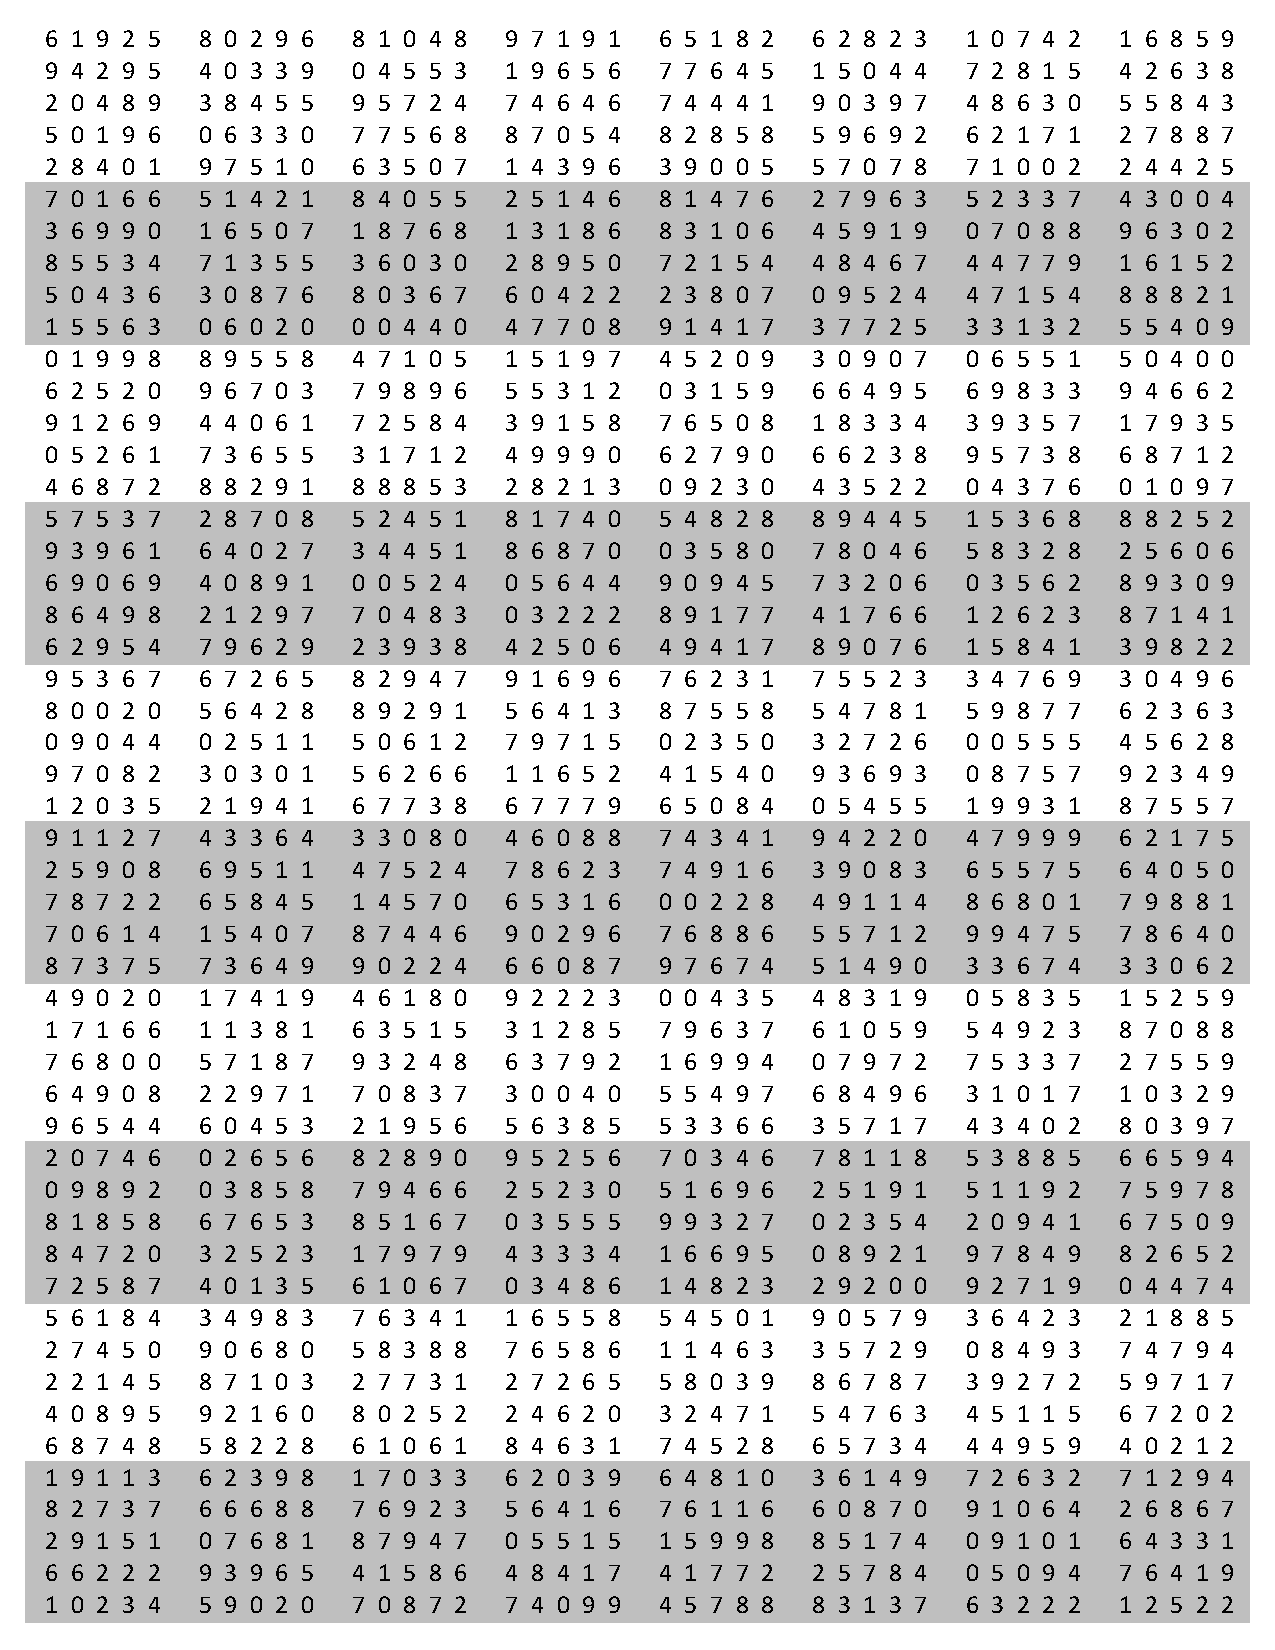
\includegraphics[width=\textwidth]{RandNumbers.pdf}



% Section 6.5 #8
\item Suppose a population has a distribution with $\mu = 72$ and $\sigma= 8$.
	\begin{enumerate}
	
	\item If we know nothing about the original population distribution and random samples of size $n=16$ are selected, why can't we say anything about the $\bar x$ distribution of sample means? 
	
	{\answer The sample size is too small to be certain what the resulting $\bar{x}$ distribution will look like.  In order to apply the Central Limit Theorem, which asserts that the $\bar{x}$ distribution is approximately normal, the sample size needs to be $n \geq 30$.
	} 

	\item If we know that the original population distribution is normal, then what can we say about the $\bar x$ distribution of random samples of $n=16$.  In this case, find $P(68 \leq \bar x \leq 73)$. 
	
	{\answer When the original population distribution is normal, then so will the $\bar{x}$ distribution, regardless of the size of the samples. 
	
	The $\bar{x}$ distribution still has a mean $\mu_{\bar{x}} = \mu = 72$, but the standard deviation is $\sigma_{\bar{x}} = \frac{\sigma}{\sqrt{n}} =\frac{8}{\sqrt{16}} = 2$. 
	
	$P(68 \leq \bar{x} \leq 73) = \texttt{normalcdf}(68, 73, 72, 2) \approx 0.6687124058$.
	} 
	
	\end{enumerate}
	
% Section 6.5 #14
\item The heights of 18-year-old men are approximately normally distributed, with a mean of 68 inches and a standard deviation of 3 inches.

	\begin{enumerate}
	
	\item What is the probability that an 18-year-old man selected at random is between 67 and 69 inches tall? 
	
	{\answer $P(67 < x < 69) = \texttt{normalcdf}(67, 69, 68, 3) \approx 0.2611171926$
	} 

	\item If a random sample of nine 18-year-old men are selected at random, what is the probability that the mean height of the sample $\bar x$ is between 67 and 69 inches? 
	
	{\answer  In this case, it is not the value of the random variable $x$ that we are considering, but rather the value of the mean $\bar{x}$ of samples of size $n = 9$.  
	
	Because the distribution of $x$ is normal, the distribution of $\bar{x}$ will be too.  Further, the mean of the $\bar{x}$ distribution is still 68, but the standard deviation of that distribution is $\frac{\sigma}{\sqrt{n}} = \frac{3}{\sqrt{9}} = 1$. 
	
	$P(67 < \bar{x} < 69) = \texttt{normalcdf}(67, 69, 68, 1) \approx 0.6826894809$
	} 

	\item Explain why the probability in part (b) is so much higher than the probability in part (a) even though they both refer to the same interval of heights (67 to 69 inches). 
	
	{\answer The standard deviation of the sample mean distribution is smaller than that of the original distribution, so there is less variance in the values.  That is, the mean height of a randomly selected sample of men is more likely to be close to the mean height of all men than a single randomly selected man's height is.
	} 
	%--
	\end{enumerate}

	
% Section 6.5 #16	
\item Let $x$ be a random variable that represents white blood cell count per cubic milliliter of whole blood.  Assume that $x$ has a distribution that is approximately normal with a mean of $\mu = 7500$ and estimated standard deviation of $\sigma = 1750$.  A test result of $x<3500$ is an indication of leukopenia.  This indicates bone marrow repression that may be the result of a viral infection.

	\begin{enumerate}
	
	\item What is the probability that, on a single test, $x$ is less than 3500? 
	
	{\answer $P(x<3500) = \texttt{normalcdf}(-1\mbox{E}99, 3500, 7500, 1750) \approx 0.01113549 \approx 1.11\%$
	} 

	\item Suppose a doctor uses the average $\bar x$ for two tests taken about a week apart.  What can we say about the probability distribution of $\bar x$?  What is the probability that $\bar x < 3500$? 
	
	{\answer Because $x$ has a distribution that is approximately normal, the distribution of the averages of the samples (even with size as small as $n=2$) is also normal.  The mean of the distribution of averages is still $7500$, however, the standard deviation is reduced to $\frac{\sigma}{\sqrt{n}} = \frac{1750}{\sqrt{2}}.$ 
	
	$P(\bar{x} < 3500) = \texttt{normalcdf}(-1\mbox{E}99, 3500, 7500, 1750/\sqrt(2)) = 0.0006135861 \approx 0.061\%$
	} 

	\item Repeat part (b) but with $n=3$ tests. 
	
	{\answer Again, the distribution of the averages of three test results is normal, with mean $7500$ and standard deviation $\frac{\sigma}{\sqrt{n}} = \frac{1750}{\sqrt{3}}$. 
	
	$P(\bar{x} < 3500) = \texttt{normalcdf}(-1\mbox{E}99, 3500, 7500, 1750\sqrt(3)) = 0.00003763633 \approx 0.0038\%$
	} 

	\item How did the probabilities change as $n$ increased?  What do such results imply about a patient that has $\bar x < 3500$ for 3 those tests?  
	
	{\answer Although it is possible for an isolated random test to indicate a low count when absolutely nothing is wrong, the greater $n$ is, it becomes less and less likely that the average of the tests will be less than 3500 when absolutely nothing is wrong. 
	
	According to part (c), the likelihood that the average of 3 tests is less than 3500 just by random chance is only $0.00003763633$.  So, for a patient with such results, the probability is extremely high that they do, in fact, have leukopenia.
	} 
	%--
	\end{enumerate}
	
%Chapter 6 Review #23-ish
\item Assume that IQ scores are normally distributed, with a standard deviation of 15 points and a mean of 100 points.  If 10 people are chosen at random, what is the probability that the sample mean of their IQ scores will not differ from the population mean by more than 2 points? 

{\answer In this case, we are looking for the probability that the sample mean $\bar{x}$ falls between 98 and 102 points.  Because the distribution of IQ scores is normal, the Central Limit Theorem can be applied with $\mu_{\bar{x}} = 100$ and $\sigma_{\bar{x}} =\frac{15}{\sqrt{10}}$. 

So, $P(98 \leq \bar{x} \leq 102) = \texttt{normalcdf}(98, 102, 100, \frac{15}{\sqrt{10}}) \approx 0.3267099507 \approx 32.67\%$.
} 

%Chapter 6 Review #24
\item A large tank of fish from a hatchery is being delivered to a lake.  The hatchery claims that the mean length of fish in the tank is 15 inches, and the standard deviation is 2 inches.  A random sample of 36 fish is taken from the tank.  Let $\bar{x}$ be the mean length of the sample.  What is the probability that $\bar{x}$ is within $0.5$ inches of the claimed population mean? 

{\answer Although there is no indication that the distribution of lengths of the fish is normal, the sample size is greater than 30, so the Central Limit Theorem applies.  So, we can apply the \texttt{normalcdf} function with $\mu_{\bar{x}}=15$ and $\sigma_{\bar{x}} = 2/\sqrt{36} = 1/3$. 

$\texttt{normalcdf(14.5, 15.5, 15, 1/3)} \approx 0.8663855426 \approx 86.64\%$
} 
\end{enumerate}
\end{document}

